%\title{Project Report}
%
%%% Preamble
\documentclass[paper=a4, fontsize=11pt]{scrartcl}
\usepackage[T1]{fontenc}
\usepackage{fourier}

\usepackage[english]{babel}															% English language/hyphenation
\usepackage[protrusion=true,expansion=true]{microtype}
\usepackage{amsmath,amsfonts,amsthm} % Math packages
\usepackage[pdftex]{graphicx}
\usepackage{url}
\usepackage{listings}
\usepackage[final]{pdfpages}
\usepackage[section]{placeins}

%%% Custom sectioning
\usepackage{sectsty}
\allsectionsfont{\centering \normalfont\scshape}


%%% Custom headers/footers (fancyhdr package)
\usepackage{fancyhdr}
\pagestyle{fancyplain}
\fancyhead{}											% No page header
\fancyfoot[L]{}											% Empty
\fancyfoot[C]{}											% Empty
\fancyfoot[R]{\thepage}									% Pagenumbering
\renewcommand{\headrulewidth}{0pt}			% Remove header underlines
\renewcommand{\footrulewidth}{0pt}				% Remove footer underlines
\setlength{\headheight}{13.6pt}


%%% Equation and float numbering
\numberwithin{equation}{section}		% Equationnumbering: section.eq#
\numberwithin{figure}{section}			% Figurenumbering: section.fig#
\numberwithin{table}{section}				% Tablenumbering: section.tab#


%%% Maketitle metadata
\newcommand{\horrule}[1]{\rule{\linewidth}{#1}} 	% Horizontal rule

\title{
		%\vspace{-1in}
		\usefont{OT1}{bch}{b}{n}
		\normalfont \normalsize \textsc{University of Michigan} \\ [25pt]
		\horrule{0.5pt} \\[0.4cm]
		\huge AERO 584, Homework  6 \\
		\horrule{2pt} \\[0.5cm]
}
\author{
		\normalfont 								\normalsize
         Huckleberry Febbo\\[-3pt]		\normalsize
        \today
}
\date{}

%%%%%%%%%%%%%%%%%%%%%%%%%%%%%%%%%%%%%%%%%%%%%%%%%%%%%%%%%%%%%%%%%%%%%
%%%%%%%%%%%%%%%%%%%%%%%%%%%%%%%%PACKAGES%%%%%%%%%%%%%%%%%%%%%%%%%%%%%%%%

% *** MATH ***
\usepackage{amsmath}
\usepackage{cases}
\usepackage{mathrsfs}
\usepackage{amssymb}
\DeclareMathAlphabet\mathbfcal{OMS}{cmsy}{b}{n}


% *** GRAPHICS ***
\usepackage[]{graphicx}
\usepackage{epstopdf}
\usepackage{svg}
\setsvg{inkscape=inkscape -z -D,svgpath=figs/}

\usepackage{lineno,hyperref}
\modulolinenumbers[5]


\bibliographystyle{elsarticle-num}
%%%%%%%%%%%%%%%%%%%%%%%

\begin{document}
\maketitle

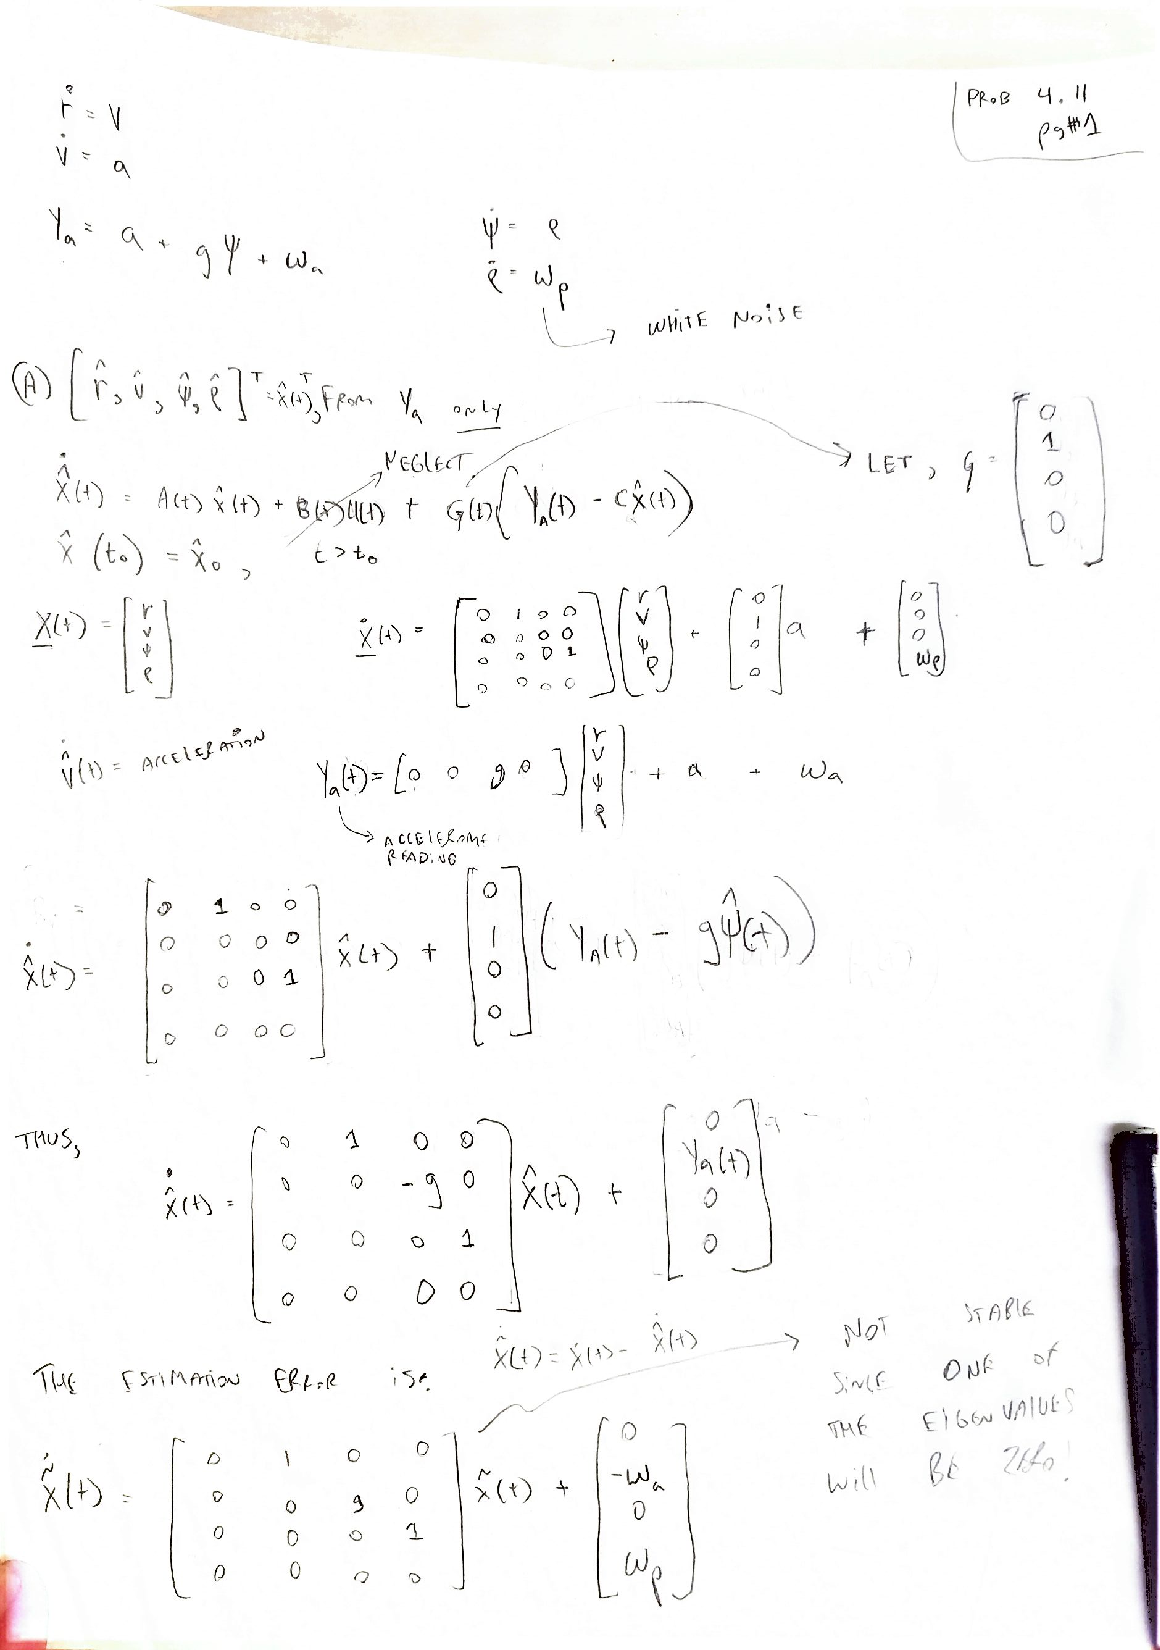
\includepdf[pages=-]{a.pdf}

%\textbf{LaTeX moved my figures, but they are all there }
\section*{Problem 4.18, Part a}


\begin{figure}[!htb]
	\centering
    \includesvg[width=0.9\textwidth]{p3_a}
	\caption{integrated $w_b$ data  using Euler's forward integration to get the Euler angles in the body frame \label{fig:f1}}
\end{figure}

\begin{figure}[!htb]
	\centering
    \includesvg[width=0.9\textwidth]{p3_a2}
	\caption{accleration in inertial frame \label{fig:f2}}
\end{figure}

\section*{Problem 4.18, Part b}
 As can be seen in Fig. \ref{fig:f3},Fig. \ref{fig:f4},Fig. \ref{fig:f5}, and Fig. \ref{fig:f6} both the velocity and position are not well captured using inertial navigation when compared to the Vicon system.
 
\begin{figure}[!htb]
	\centering
    \includesvg[width=0.9\textwidth]{p3_a3}
	\caption{ \label{fig:f3}}
\end{figure}
\begin{figure}[!htb]
	\centering
    \includesvg[width=0.9\textwidth]{p3_a4}
	\caption{ \label{fig:f4}}
\end{figure}
\begin{figure}[!htb]
	\centering
    \includesvg[width=0.9\textwidth]{p3_a5}
	\caption{ \label{fig:f5}}
\end{figure}
\begin{figure}[!htb]
	\centering
    \includesvg[width=0.9\textwidth]{p3_a6}
	\caption{ \label{fig:f6}}
\end{figure}

\section*{Problem 4.18, Part c}
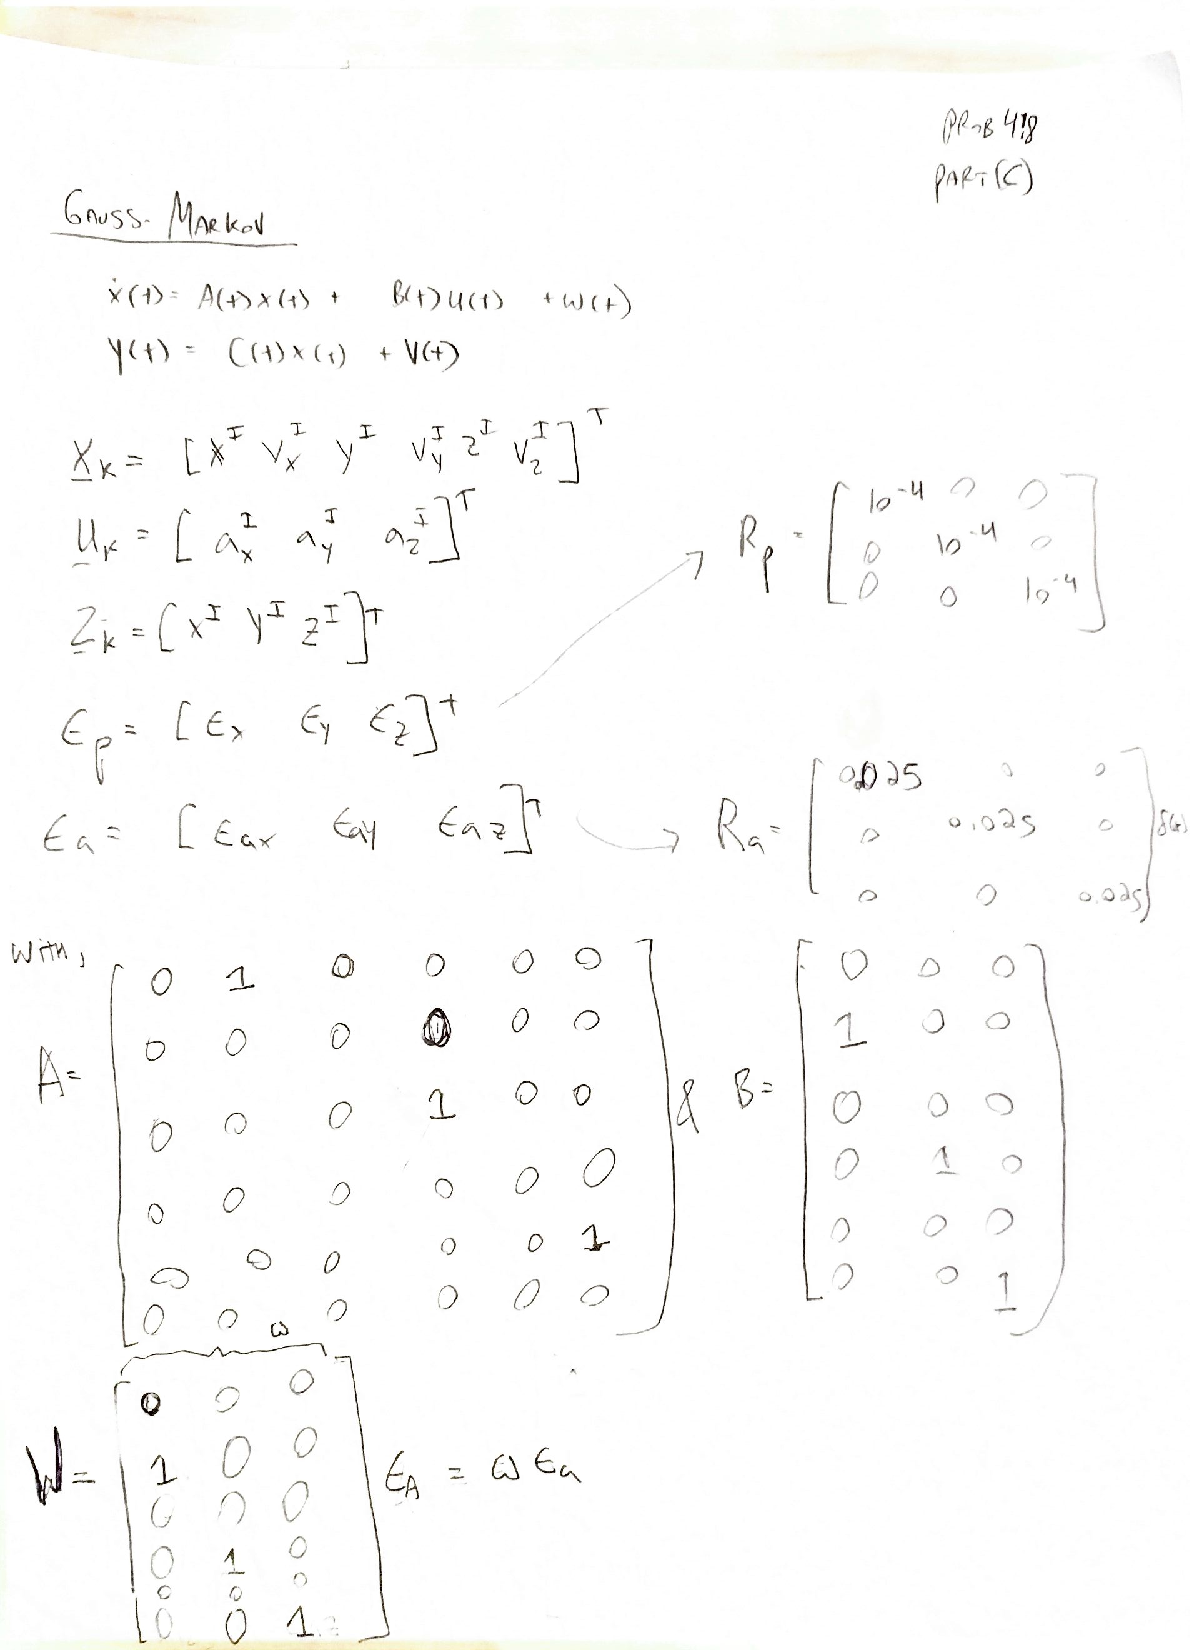
\includepdf[pages=-]{y.pdf}

The Kalman Filter does a nice job, all of the plots are zoomed in because the inertial n
\begin{figure}[!htb]
	\centering
    \includesvg[width=0.9\textwidth]{p3_a7}
	\caption{ \label{fig:f7}}
\end{figure}

\begin{figure}[!htb]
	\centering
    \includesvg[width=0.9\textwidth]{p3_a8}
	\caption{ \label{fig:f8}}
\end{figure}

\begin{figure}[!htb]
	\centering
    \includesvg[width=0.9\textwidth]{p3_a9}
	\caption{ \label{fig:f9}}
\end{figure}


\begin{figure}[!htb]
	\centering
    \includesvg[width=0.9\textwidth]{p3_a10}
	\caption{ \label{fig:f10}}
\end{figure}

\section*{Problem 4.18, Part d i}

Using this much higher covariance significantly decreases performance.
\begin{figure}[!htb]
	\centering
    \includesvg[width=0.7\textwidth]{p3_a11}
	\caption{ \label{fig:f11}}
\end{figure}

\section*{Problem 4.18, Part d ii}
While case ii is better than case i, it is not really any better than the original Filter that was designed.

\begin{figure}[!htb]
	\centering
    \includesvg[width=0.7\textwidth]{p3_a12}
	\caption{ \label{fig:f12}}
\end{figure}

\section*{Problem 4.18, Part e i and e ii}
Less frequent updates has a significant impact on the x and y states. 

\begin{figure}[!htb]
	\centering
    \includesvg[width=0.7\textwidth]{p3_a13}
	\caption{ \label{fig:f13}}
\end{figure}


\section*{Problem 4.18, julia code}
\begin{lstlisting}
using Plots
pgfplots()
using LaTeXStrings
PGFPlots.pushPGFPlotsPreamble("\\usepackage{amssymb}")
using Interpolations
using OrdinaryDiffEq
using DiffEqBase
using DataFrames

d = readtable("data.csv")

# extract data
t = d[:t]/1000; # convert to seconds
xi = d[:xi]
yi = d[:yi]
zi = d[:zi]
q_x = d[:q_x]
q_y = d[:q_y]
q_z = d[:q_z]
q_w = d[:q_w]
ax_b = d[:ax_b]
ay_b = d[:ay_b]
az_b = d[:az_b]
wx_b = d[:wx_b]
wy_b = d[:wy_b]
wz_b = d[:wz_b]

# misc variables
L = length(wz_b)
s1 = ""
l1 = (4,:red,:solid)

#s2 = "asmptotic observer"
l2 = (3,:green,:solid)

#s3 = "input"
l3 = (2.2,:black,:dash)

l4 = (1.5,:blue,:dot)

# rotation matrix, https://en.wikipedia.org/wiki/Conversion_between_quaternions_and_Euler_angles
function R(q_x,q_y,q_z,q_w)
   [1 - 2*(q_y^2 + q_z^2)       2*(q_x*q_y - q_w*q_z)     2*(q_w*q_y + q_x*q_z);
    2*(q_x*q_y + q_w*q_z)       1-2*(q_x^2 + q_z^2)       2*(q_z*q_y - q_w*q_x);
    2*(q_x*q_z - q_w*q_y)       2*(q_z*q_y + q_w*q_x)     1-2*(q_y^2 + q_x^2)];
end

# direction cosine matrices, 3-2-1 sequence (psi,theta,phi)
# [x,y,z] = Rz(psi)*Ry(theta)*Rz(phi)[X;Y;Z]
function Rz(psi)
 [cos(psi) -sin(psi) 0;
  sin(psi)  cos(psi) 0;
     0         0     1]
end

function Ry(theta)
 [cos(theta)       0   sin(theta);
      0            1       0;
  -sin(theta)      0     cos(theta)]
end

function Rx(phi)
 [1         0       0;
  0       cos(phi) -sin(phi);
  0       sin(phi)  cos(phi)]
end

##################
# part a)
psi_b = zeros(L); psi_b[1] = 0;
theta_b = zeros(L); theta_b[1] = 0;
phi_b = zeros(L); phi_b[1] = pi/2;

# integrated w_b data  using Euler's forward integration to get the Euler angles in the body frame
for i in 1:L-1
 psi_b[i+1] = psi_b[i] + wx_b[i]*(t[i+1] - t[i])
 theta_b[i+1] = theta_b[i] + wy_b[i]*(t[i+1] - t[i])
 phi_b[i+1] = phi_b[i] + wz_b[i]*(t[i+1] - t[i])
end

# find accleration in inertial frame
ax = zeros(L)
ay = zeros(L)
az = zeros(L)

for i in 1:L-1
 ab = [ax_b[i];ay_b[i];az_b[i]]
 a = Rx(phi_b[i])*Ry(theta_b[i])*Rz(psi_b[i])*ab + [0;0;-9.8]
 ax[i] = a[1]; ay[i] = a[2]; az[i] = a[3];
end

# angular velocity plots
p1 = plot(t,psi_b,line=l1,label=s1)
yaxis!(string(" ",L"$\psi$"))
xaxis!("Time (s)")

p2 = plot(t,theta_b,line=l1,label=s1)
yaxis!(string(" ",L"$\theta$"))
xaxis!("Time (s)")

p3 = plot(t,phi_b,line=l1,label=s1)
yaxis!(string(" ",L"$\phi$"))
xaxis!("Time (s)")

plot(p1,p2,p3,layout=@layout([a;b;c]),size=[600,600])

savefig(string("figs/p3_a",".",:svg));

# inertial acceleration plots
p1 = plot(t,ax,line=l1,label=s1)
yaxis!(string("ax, ",L"$\frac{m}{s^2}$"))
xaxis!("Time (s)")

p2 = plot(t,ay,line=l1,label=s1)
yaxis!(string("ay, ",L"$\frac{m}{s^2}$"))
xaxis!("Time (s)")

p3 = plot(t,az,line=l1,label=s1)
yaxis!(string("az, ",L"$\frac{m}{s^2}$"))
xaxis!("Time (s)")

pap = plot(p1,p2,p3,layout=@layout([a;b;c]),size=[600,600])

savefig(string("figs/p3_a2",".",:svg));

##################
# part b)
X0 = [-1.53; -1.5; 1.58]
V0 = [0; 0; 0]

x_in = zeros(L); x_in[1] = X0[1];
y_in = zeros(L); y_in[1] = X0[2];
z_in = zeros(L); z_in[1] = X0[3];
vx_in = zeros(L); vx_in[1] = V0[1];
vy_in = zeros(L); vy_in[1] = V0[2];
vz_in = zeros(L); vz_in[1] = V0[3];

# integrate using inertial navigation
for i in 1:L-1
 vx_in[i+1] = vx_in[i] + ax[i]*(t[i+1] - t[i])
 vy_in[i+1] = vy_in[i] + ay[i]*(t[i+1] - t[i])
 vz_in[i+1] = vz_in[i] + az[i]*(t[i+1] - t[i])
 x_in[i+1] = x_in[i] + vx_in[i]*(t[i+1] - t[i])
 y_in[i+1] = y_in[i] + vy_in[i]*(t[i+1] - t[i])
 z_in[i+1] = z_in[i] + vz_in[i]*(t[i+1] - t[i])
end

# differentiate Vicon position data
vxi = zeros(L)
vyi = zeros(L)
vzi = zeros(L)

for i in 1:L-1
 vxi[i] = (xi[i+1] - xi[i])*(t[i+1] - t[i])
 vyi[i] = (yi[i+1] - yi[i])*(t[i+1] - t[i])
 vzi[i] = (zi[i+1] - zi[i])*(t[i+1] - t[i])
end

s1 = "inertial navigation"
s2 = "using Vicon"

# position
p1 = plot(t,x_in,line=l1,label=s1)
plot!(t,xi,line=l2,label=s2)
yaxis!("x (m)")
xaxis!("Time (s)")

p2 = plot(t,y_in,line=l1,label=s1)
plot!(t,yi,line=l2,label=s2)
yaxis!("y (m)")
xaxis!("Time (s)")

p3 = plot(t,z_in,line=l1,label=s1)
plot!(t,zi,line=l2,label=s2)
yaxis!("z (m)")
xaxis!("Time (s)")

plot(p1,p2,p3,layout=@layout([a;b;c]),size=[600,600])

savefig(string("figs/p3_a3",".",:svg));

plot(x_in,y_in,z_in,line=l1,label=s1,cbar=false)
plot!(xi,yi,zi,line=l2,label=s2,cbar=false,size=[800,800])
xaxis!("x (m)")
yaxis!("y (m)")
savefig(string("figs/p3_a4",".",:svg));

# velocity
p1 = plot(t,vx_in,line=l1,label=s1)
plot!(t,vxi,line=l2,label=s2)
yaxis!("vx (m/s)")
xaxis!("Time (s)")

p2 = plot(t,vy_in,line=l1,label=s1)
plot!(t,vyi,line=l2,label=s2)
yaxis!("vy (m/s)")
xaxis!("Time (s)")

p3 = plot(t,vz_in,line=l1,label=s1)
plot!(t,vzi,line=l2,label=s2)
yaxis!("vz (m/s)")
xaxis!("Time (s)")

plot(p1,p2,p3,layout=@layout([a;b;c]),size=[600,600])

savefig(string("figs/p3_a5",".",:svg));

plot(vx_in,vy_in,vz_in,line=l1,label=s1,cbar=false)
plot!(vxi,vyi,vzi,line=l2,label=s2,cbar=false,size=[800,800])
xaxis!("vx (m/s)")
yaxis!("vy (m/s)")
savefig(string("figs/p3_a6",".",:svg));

##################
# part c)
# calculate a using quaternion data from Vicon system
axi = zeros(L)
ayi = zeros(L)
azi = zeros(L)

for i in 1:L-1
 ab = [ax_b[i];ay_b[i];az_b[i]]
 a = R(q_x[i],q_y[i],q_z[i],q_w[i])*ab + [0;0;-9.8]
 axi[i] = a[1]; ayi[i] = a[2]; azi[i] = a[3];
end

# inertial acceleration plots
p1 = plot(t,ax,line=l1,label=s1)
plot!(t,axi,line=l2,label=s2)
yaxis!(string("ax, ",L"$\frac{m}{s^2}$"))
xaxis!("Time (s)")

p2 = plot(t,ay,line=l1,label=s1)
plot!(t,ayi,line=l2,label=s2)
yaxis!(string("ay, ",L"$\frac{m}{s^2}$"))
xaxis!("Time (s)")

p3 = plot(t,az,line=l1,label=s1)
plot!(t,azi,line=l2,label=s2)
yaxis!(string("az, ",L"$\frac{m}{s^2}$"))
xaxis!("Time (s)")

plot(p1,p2,p3,layout=@layout([a;b;c]),size=[600,600])

savefig(string("figs/p3_a7",".",:svg));

# Kalman Filter
v = eye(3)
w = [0 0 0;
     1 0 0;
     0 0 0;
     0 1 0;
     0 0 0;
     0 0 1]
Ra = eye(3)*10.0^(-4)
Rp = eye(3)*0.025
Rw = w*Rp*w'
Rv = v*Ra*v'

x_k = zeros(L); x_k[1] = X0[1];
y_k = zeros(L); y_k[1] = X0[2];
z_k = zeros(L); z_k[1] = X0[3];
vx_k = zeros(L); vx_k[1] = V0[1];
vy_k = zeros(L); vy_k[1] = V0[2];
vz_k = zeros(L); vz_k[1] = V0[3];

x = zeros(L,6); x[1,1:3] = X0; x[1,4:6] = V0;
P = zeros(L,6,6)
for i in 1:L-1
 dt = d[:t][i+1] - d[:t][i]
 A = [1 dt 0  0  0  0;
      0  1 0  0  0  0;
      0  0  1 dt 0  0;
      0  0  0  1  0 0;
      0  0  0  0  1 dt;
      0  0  0  0  0  1]

 B = [0   0  0;
      dt  0  0;
      0   0  0;
      0  dt  0;
      0   0  0;
      0   0  dt]

 C = [1 dt 0 0  0  0;
      0 0  1 dt 0  0;
      0 0  0 0  1  dt]

 # time update (predict)
 u = [axi[i];ayi[i];azi[i]]
 x[i+1,:] = A*x[i,:] + B*u
 P[i+1,:,:] = A*P[i,:,:]*A' + Rw

 # measurment update
 y = [xi[i];yi[i];zi[i]]
 K = P[i+1,:,:]*C'*inv((C*P[i+1,:,:]*C' + Rv))
 x[i+1,:] = x[i+1,:] + K*(y-C*x[i+1,:])
 P[i+1,:,:] = (eye(6) - K*C)*P[i+1,:,:]

 # save results
 x_k[i+1] = x[i+1,1]
 vx_k[i+1] = x[i+1,2]

 y_k[i+1] = x[i+1,3]
 vy_k[i+1] = x[i+1,4]

 z_k[i+1] = x[i+1,5]
 vz_k[i+1] = x[i+1,6]
end

s1 = "inertial navigation"
s2 = "using Vicon"
s3 = "Kalman Filter"

# position
p1 = plot(t,x_in,line=l1,label=s1)
plot!(t,xi,line=l2,label=s2)
plot!(t,x_k,line=l3,label=s3)
yaxis!("x (m)")
xaxis!("Time (s)")
ylims!(-5,5);

p2 = plot(t,y_in,line=l1,label=s1)
plot!(t,yi,line=l2,label=s2)
plot!(t,y_k,line=l3,label=s3)
yaxis!("y (m)")
xaxis!("Time (s)")
ylims!(-5,5);

p3 = plot(t,z_in,line=l1,label=s1)
plot!(t,zi,line=l2,label=s2)
plot!(t,z_k,line=l3,label=s3)
yaxis!("z (m)")
xaxis!("Time (s)")
ylims!(-5,5);

plot(p1,p2,p3,layout=@layout([a;b;c]),size=[600,600])

savefig(string("figs/p3_a8",".",:svg));

#plot(x_in,y_in,z_in,line=l1,label=s1,cbar=false)
plot(xi,yi,zi,line=l2,label=s2,cbar=false)
plot!(x_k,y_k,z_k,line=l3,label=s3,cbar=false,size=[800,800])
xaxis!("x (m)")
yaxis!("y (m)")
savefig(string("figs/p3_a9",".",:svg));

# velocity
p1 = plot(t,vx_in,line=l1,label=s1)
plot!(t,vxi,line=l2,label=s2)
plot!(t,vx_k,line=l3,label=s3)
yaxis!("vx (m/s)")
xaxis!("Time (s)")
ylims!(-1,1);

p2 = plot(t,vy_in,line=l1,label=s1)
plot!(t,vyi,line=l2,label=s2)
plot!(t,vy_k,line=l3,label=s3)
yaxis!("vy (m/s)")
xaxis!("Time (s)")
ylims!(-1,1);

p3 = plot(t,vz_in,line=l1,label=s1)
plot!(t,vzi,line=l2,label=s2)
plot!(t,vz_k,line=l3,label=s3)
yaxis!("vz (m/s)")
xaxis!("Time (s)")
ylims!(-1,1);

plot(p1,p2,p3,layout=@layout([a;b;c]),size=[600,600])

savefig(string("figs/p3_a10",".",:svg));

##################
# part d) i
Ra =[2.5  0  0;
     0   2.5 0;
     0    0  2.5]

s1 = "using Vicon"
s2 = "Kalman Filter, part c"
s3 = "Kalman Filter, part d-i"
s4 = "Kalman Filter, part d-ii"

# Kalman Filter
v = eye(3)
w = [0 0 0;
     1 0 0;
     0 0 0;
     0 1 0;
     0 0 0;
     0 0 1]
#Ra = eye(3)*10.0^(-4)
Rp = eye(3)*0.025
Rw = w*Rp*w'
Rv = v*Ra*v'

x_k2 = zeros(L); x_k[1] = X0[1];
y_k2 = zeros(L); y_k[1] = X0[2];
z_k2 = zeros(L); z_k[1] = X0[3];
vx_k2 = zeros(L); vx_k[1] = V0[1];
vy_k2 = zeros(L); vy_k[1] = V0[2];
vz_k2 = zeros(L); vz_k[1] = V0[3];

x = zeros(L,6); x[1,1:3] = X0; x[1,4:6] = V0;
P = zeros(L,6,6)
for i in 1:L-1
 dt = d[:t][i+1] - d[:t][i]
 A = [1 dt 0  0  0  0;
      0  1 0  0  0  0;
      0  0  1 dt 0  0;
      0  0  0  1  0 0;
      0  0  0  0  1 dt;
      0  0  0  0  0  1]

 B = [0   0  0;
      dt  0  0;
      0   0  0;
      0  dt  0;
      0   0  0;
      0   0  dt]

 C = [1 dt 0 0  0  0;
      0 0  1 dt 0  0;
      0 0  0 0  1  dt]

 # time update (predict)
 u = [axi[i];ayi[i];azi[i]]
 x[i+1,:] = A*x[i,:] + B*u
 P[i+1,:,:] = A*P[i,:,:]*A' + Rw

 # measurment update
 y = [xi[i];yi[i];zi[i]]
 K = P[i+1,:,:]*C'*inv((C*P[i+1,:,:]*C' + Rv))
 x[i+1,:] = x[i+1,:] + K*(y-C*x[i+1,:])
 P[i+1,:,:] = (eye(6) - K*C)*P[i+1,:,:]

 # save results
 x_k2[i+1] = x[i+1,1]
 vx_k2[i+1] = x[i+1,2]

 y_k2[i+1] = x[i+1,3]
 vy_k2[i+1] = x[i+1,4]

 z_k2[i+1] = x[i+1,5]
 vz_k2[i+1] = x[i+1,6]
end

# position
p1 = plot(t,xi,line=l1,label=s1)
plot!(t,x_k,line=l2,label=s2)
plot!(t,x_k2,line=l3,label=s3)
yaxis!("x (m)")
xaxis!("Time (s)")
ylims!(-5,5);

p2 = plot(t,yi,line=l1,label=s1)
plot!(t,y_k,line=l2,label=s2)
plot!(t,y_k2,line=l3,label=s3)
yaxis!("y (m)")
xaxis!("Time (s)")
ylims!(-5,5);

p3 = plot(t,zi,line=l1,label=s1)
plot!(t,z_k,line=l2,label=s2)
plot!(t,z_k2,line=l3,label=s3)
yaxis!("z (m)")
xaxis!("Time (s)")
ylims!(-5,5);

# velocity
p4 = plot(t,vxi,line=l1,label=s1)
plot!(t,vx_k,line=l2,label=s2)
plot!(t,vx_k2,line=l3,label=s3)
yaxis!("vx (m/s)")
xaxis!("Time (s)")
ylims!(-1,1);

p5 = plot(t,vyi,line=l1,label=s1)
plot!(t,vy_k,line=l2,label=s2)
plot!(t,vy_k2,line=l3,label=s3)
yaxis!("vy (m/s)")
xaxis!("Time (s)")
ylims!(-1,1);

p6 = plot(t,vzi,line=l1,label=s1)
plot!(t,vz_k,line=l2,label=s2)
plot!(t,vz_k2,line=l3,label=s3)
yaxis!("vz (m/s)")
xaxis!("Time (s)")
ylims!(-1,1);

plot(p1,p2,p3,p4,p5,p6,layout=@layout([a;b;c;d;e;f]),size=[600,1000])

savefig(string("figs/p3_a11",".",:svg));

##################
# part d) ii
Ra = eye(3)*2.5^(-4)

s1 = "using Vicon"
s2 = "Kalman Filter, part c"
s3 = "Kalman Filter, part d-i"
s4 = "Kalman Filter, part d-ii"

# Kalman Filter
v = eye(3)
w = [0 0 0;
     1 0 0;
     0 0 0;
     0 1 0;
     0 0 0;
     0 0 1]
#Ra = eye(3)*10.0^(-4)
Rp = eye(3)*0.025
Rw = w*Rp*w'
Rv = v*Ra*v'

x_k3 = zeros(L); x_k[1] = X0[1];
y_k3 = zeros(L); y_k[1] = X0[2];
z_k3 = zeros(L); z_k[1] = X0[3];
vx_k3 = zeros(L); vx_k[1] = V0[1];
vy_k3 = zeros(L); vy_k[1] = V0[2];
vz_k3 = zeros(L); vz_k[1] = V0[3];

x = zeros(L,6); x[1,1:3] = X0; x[1,4:6] = V0;
P = zeros(L,6,6)
for i in 1:L-1
 dt = d[:t][i+1] - d[:t][i]
 A = [1 dt 0  0  0  0;
      0  1 0  0  0  0;
      0  0  1 dt 0  0;
      0  0  0  1  0 0;
      0  0  0  0  1 dt;
      0  0  0  0  0  1]

 B = [0   0  0;
      dt  0  0;
      0   0  0;
      0  dt  0;
      0   0  0;
      0   0  dt]

 C = [1 dt 0 0  0  0;
      0 0  1 dt 0  0;
      0 0  0 0  1  dt]

 # time update (predict)
 u = [axi[i];ayi[i];azi[i]]
 x[i+1,:] = A*x[i,:] + B*u
 P[i+1,:,:] = A*P[i,:,:]*A' + Rw

 # measurment update
 y = [xi[i];yi[i];zi[i]]
 K = P[i+1,:,:]*C'*inv((C*P[i+1,:,:]*C' + Rv))
 x[i+1,:] = x[i+1,:] + K*(y-C*x[i+1,:])
 P[i+1,:,:] = (eye(6) - K*C)*P[i+1,:,:]

 # save results
 x_k3[i+1] = x[i+1,1]
 vx_k3[i+1] = x[i+1,2]

 y_k3[i+1] = x[i+1,3]
 vy_k3[i+1] = x[i+1,4]

 z_k3[i+1] = x[i+1,5]
 vz_k3[i+1] = x[i+1,6]
end

# position
p1 = plot(t,xi,line=l1,label=s1)
plot!(t,x_k,line=l2,label=s2)
plot!(t,x_k2,line=l3,label=s3)
plot!(t,x_k3,line=l4,label=s4)
yaxis!("x (m)")
xaxis!("Time (s)")
ylims!(-5,5);

p2 = plot(t,yi,line=l1,label=s1)
plot!(t,y_k,line=l2,label=s2)
plot!(t,y_k2,line=l3,label=s3)
plot!(t,y_k3,line=l4,label=s4)
yaxis!("y (m)")
xaxis!("Time (s)")
ylims!(-5,5);

p3 = plot(t,zi,line=l1,label=s1)
plot!(t,z_k,line=l2,label=s2)
plot!(t,z_k2,line=l3,label=s3)
plot!(t,z_k3,line=l4,label=s4)
yaxis!("z (m)")
xaxis!("Time (s)")
ylims!(-5,5);

# velocity
p4 = plot(t,vxi,line=l1,label=s1)
plot!(t,vx_k,line=l2,label=s2)
plot!(t,vx_k2,line=l3,label=s3)
plot!(t,vx_k3,line=l4,label=s4)
yaxis!("vx (m/s)")
xaxis!("Time (s)")
ylims!(-1,1);

p5 = plot(t,vyi,line=l1,label=s1)
plot!(t,vy_k,line=l2,label=s2)
plot!(t,vy_k2,line=l3,label=s3)
plot!(t,vy_k3,line=l4,label=s4)
yaxis!("vy (m/s)")
xaxis!("Time (s)")
ylims!(-1,1);

p6 = plot(t,vzi,line=l1,label=s1)
plot!(t,vz_k,line=l2,label=s2)
plot!(t,vz_k2,line=l3,label=s3)
plot!(t,vz_k3,line=l4,label=s4)
yaxis!("vz (m/s)")
xaxis!("Time (s)")
ylims!(-1,1);

plot(p1,p2,p3,p4,p5,p6,layout=@layout([a;b;c;d;e;f]),size=[600,1000])

savefig(string("figs/p3_a12",".",:svg));


##################
# part e) i

# Kalman Filter
v = eye(3)
w = [0 0 0;
     1 0 0;
     0 0 0;
     0 1 0;
     0 0 0;
     0 0 1]
Ra = eye(3)*10.0^(-4)
Rp = eye(3)*0.025
Rw = w*Rp*w'
Rv = v*Ra*v'

x_k2 = zeros(L); x_k[1] = X0[1];
y_k2 = zeros(L); y_k[1] = X0[2];
z_k2 = zeros(L); z_k[1] = X0[3];
vx_k2 = zeros(L); vx_k[1] = V0[1];
vy_k2 = zeros(L); vy_k[1] = V0[2];
vz_k2 = zeros(L); vz_k[1] = V0[3];

x = zeros(L,6); x[1,1:3] = X0; x[1,4:6] = V0;
P = zeros(L,6,6)
for i in 1:L-1
 dt = d[:t][i+1] - d[:t][i]
 A = [1 dt 0  0  0  0;
      0  1 0  0  0  0;
      0  0  1 dt 0  0;
      0  0  0  1  0 0;
      0  0  0  0  1 dt;
      0  0  0  0  0  1]

 B = [0   0  0;
      dt  0  0;
      0   0  0;
      0  dt  0;
      0   0  0;
      0   0  dt]

 C = [1 dt 0 0  0  0;
      0 0  1 dt 0  0;
      0 0  0 0  1  dt]

 # time update (predict)
 u = [axi[i];ayi[i];azi[i]]
 x[i+1,:] = A*x[i,:] + B*u
 P[i+1,:,:] = A*P[i,:,:]*A' + Rw

 # measurment update
 if i==1 || (i-1) % 3 == 0
  y = [xi[i];yi[i];zi[i]]
 end
 K = P[i+1,:,:]*C'*inv((C*P[i+1,:,:]*C' + Rv))
 x[i+1,:] = x[i+1,:] + K*(y-C*x[i+1,:])
 P[i+1,:,:] = (eye(6) - K*C)*P[i+1,:,:]

 # save results
 x_k2[i+1] = x[i+1,1]
 vx_k2[i+1] = x[i+1,2]

 y_k2[i+1] = x[i+1,3]
 vy_k2[i+1] = x[i+1,4]

 z_k2[i+1] = x[i+1,5]
 vz_k2[i+1] = x[i+1,6]
end


##################
# part e) ii

# Kalman Filter
v = eye(3)
w = [0 0 0;
     1 0 0;
     0 0 0;
     0 1 0;
     0 0 0;
     0 0 1]
Ra = eye(3)*10.0^(-4)
Rp = eye(3)*0.025
Rw = w*Rp*w'
Rv = v*Ra*v'

x_k3 = zeros(L); x_k[1] = X0[1];
y_k3 = zeros(L); y_k[1] = X0[2];
z_k3 = zeros(L); z_k[1] = X0[3];
vx_k3 = zeros(L); vx_k[1] = V0[1];
vy_k3 = zeros(L); vy_k[1] = V0[2];
vz_k3 = zeros(L); vz_k[1] = V0[3];

x = zeros(L,6); x[1,1:3] = X0; x[1,4:6] = V0;
P = zeros(L,6,6)
for i in 1:L-1
 dt = d[:t][i+1] - d[:t][i]
 A = [1 dt 0  0  0  0;
      0  1 0  0  0  0;
      0  0  1 dt 0  0;
      0  0  0  1  0 0;
      0  0  0  0  1 dt;
      0  0  0  0  0  1]

 B = [0   0  0;
      dt  0  0;
      0   0  0;
      0  dt  0;
      0   0  0;
      0   0  dt]

 C = [1 dt 0 0  0  0;
      0 0  1 dt 0  0;
      0 0  0 0  1  dt]

 # time update (predict)
 u = [axi[i];ayi[i];azi[i]]
 x[i+1,:] = A*x[i,:] + B*u
 P[i+1,:,:] = A*P[i,:,:]*A' + Rw

 # measurment update
 if i==1 || (i-1) % 10 == 0
  y = [xi[i];yi[i];zi[i]]
 end
 K = P[i+1,:,:]*C'*inv((C*P[i+1,:,:]*C' + Rv))
 x[i+1,:] = x[i+1,:] + K*(y-C*x[i+1,:])
 P[i+1,:,:] = (eye(6) - K*C)*P[i+1,:,:]

 # save results
 x_k3[i+1] = x[i+1,1]
 vx_k3[i+1] = x[i+1,2]

 y_k3[i+1] = x[i+1,3]
 vy_k3[i+1] = x[i+1,4]

 z_k3[i+1] = x[i+1,5]
 vz_k3[i+1] = x[i+1,6]
end

s1 = "using Vicon"
s2 = "Kalman Filter, part c"
s3 = "updated every 3rd"
s4 = "udated every 10th"

# position
p1 = plot(t,xi,line=l1,label=s1)
plot!(t,x_k,line=l2,label=s2)
plot!(t,x_k2,line=l3,label=s3)
plot!(t,x_k3,line=l4,label=s4)
yaxis!("x (m)")
xaxis!("Time (s)")
ylims!(-5,5);

p2 = plot(t,yi,line=l1,label=s1)
plot!(t,y_k,line=l2,label=s2)
plot!(t,y_k2,line=l3,label=s3)
plot!(t,y_k3,line=l4,label=s4)
yaxis!("y (m)")
xaxis!("Time (s)")
ylims!(-5,5);

p3 = plot(t,zi,line=l1,label=s1)
plot!(t,z_k,line=l2,label=s2)
plot!(t,z_k2,line=l3,label=s3)
plot!(t,z_k3,line=l4,label=s4)
yaxis!("z (m)")
xaxis!("Time (s)")
ylims!(-5,5);

# velocity
p4 = plot(t,vxi,line=l1,label=s1)
plot!(t,vx_k,line=l2,label=s2)
plot!(t,vx_k2,line=l3,label=s3)
plot!(t,vx_k3,line=l4,label=s4)
yaxis!("vx (m/s)")
xaxis!("Time (s)")
ylims!(-.1,.1);

p5 = plot(t,vyi,line=l1,label=s1)
plot!(t,vy_k,line=l2,label=s2)
plot!(t,vy_k2,line=l3,label=s3)
plot!(t,vy_k3,line=l4,label=s4)
yaxis!("vy (m/s)")
xaxis!("Time (s)")
ylims!(-.1,.1);

p6 = plot(t,vzi,line=l1,label=s1)
plot!(t,vz_k,line=l2,label=s2)
plot!(t,vz_k2,line=l3,label=s3)
plot!(t,vz_k3,line=l4,label=s4)
yaxis!("vz (m/s)")
xaxis!("Time (s)")
ylims!(-.1,.1);

plot(p1,p2,p3,p4,p5,p6,layout=@layout([a;b;c;d;e;f]),size=[600,1000])

savefig(string("figs/p3_a13",".",:svg));

\end{lstlisting}

\end{document}
